\documentclass[a4paper, 11pt,reqno]{article}
\input{/Users/olivierglorieux/Desktop/BCPST/2020:2021/preambule.tex}
\usepackage{enumitem}
\geometry{hmargin=2.5cm, vmargin=2.5cm}
\lstset{basicstyle=\ttfamily, keywordstyle=\rmfamily\bfseries}
\newif\ifshow
\showtrue
\input{/Users/olivierglorieux/Desktop/BCPST/2021:2022/ifshow.tex}

\author{Olivier Glorieux}


\begin{document}

\title{Corrections - Révisions Pâques
}

\section{Complexes}





%-------------------------------------------------------------
%-------------------------------------------------------------
%-------------------------------------------------------------
%-------------------------------------------------------------
%-------------------------------------------------------------
%-------------------------------------------------------------




\begin{exercice}
Soit $\bU$ l'ensemble des complexes de module $1$. 
\begin{enumerate}
\item Calculer 
$$\inf \left\{ \left| \frac{1}{z}+z\right| , z \in \bU\right\}$$

\item Pour tout $z\in \bC^*$ on note  $\alpha(z)= \frac{1}{\bar{z}}+z$. 
\begin{enumerate}
\item Calculer le module de $\alpha(z)$ en fonction de celui de $z$. 
\item Montrer que pour tout $x>0$ on a : $\ddp \frac{1}{x}+x\geq 2$.
\item En déduire 
$$\inf\{ \left| \alpha(z)\right| , z \in \bC^*\}$$
\end{enumerate}
\end{enumerate}
\end{exercice}


\begin{correction}
\begin{enumerate}
\item Comme $z\in \bU$, il existe $\theta\in [0,2\pi[$ tel que $z=e^{i\theta}$. 
Donc 
\begin{align*}
\left| \frac{1}{z}+z\right| &= \left|e^{-i\theta} +e^{i\theta}\right|\\
									&=  \left|2\cos(\frac{\theta}{2}\right|
\end{align*}

Pour $\theta =\pi $ on a $ \left|2\cos(\frac{\theta}{2}\right| =0$ donc 
$$\inf \left\{ \left| \frac{1}{z}+z\right| , z \in \bU\right\}=0$$

\item 
\begin{enumerate}
\item \begin{align*}
 \left| \alpha(z)\right|  &= \left|  \frac{1}{\bar{z}}+z\right|  \\
 								&=  \left|  \frac{1+z\bar{z}}{\bar{z}}\right|  \\	 												&=  \left|  \frac{1+|z|^2}{\bar{z}}\right|  \\
								&=   \frac{|1+|z|^2|}{|\bar{z}|}\\ 								
								&=   \frac{1+|z|^2}{|z|}\\ 								 												&=   \frac{1}{|z|}+|z| 								 							
\end{align*}
\item Pour tout $x>0$ on a 
\begin{align*}
x+\frac{1}{x}-2 &=\frac{x^2-2x+1}{x}\\
						&=\frac{(x-1)^2}{x}\geq 0\\
\end{align*}
Donc pour tout $x>0$, $x+\frac{1}{x}-2 \geq 0$. 
\item 
On a $ \left| \alpha(1)\right|  = \frac{1}{|1|}+|1|=2$ et on a vu que 
pour tout $z\in \bC^*$,   $\left| \alpha(z)\right| \geq 2$ donc 
$$\inf\{ \left| \alpha(z)\right| , z \in \bC^*\}=2$$
\end{enumerate}
\end{enumerate}


\end{correction}



\begin{exercice}
On considère l'équation suivante , d'inconnue $z\in \bC$ : 
\begin{equation}\tag{$E$}
z^3 +z+1=0
\end{equation} 



%\paragraph{Partie II : Cas n=3}
\begin{enumerate}
\item On note $f : \R\mapsto \R, $ la fonciton définie par $f(t) = t^3+t+1.$
A l'aide de l'étude de $f$, justifier que l'équation $(E)$ possède une unique solution réelle, que l'on notera $r$. Montrer que $r \in ]-1, \frac{-1}{2}[$.
\item On note $z_1$ et $z_2$ les deux autres solutions complexes de $(E)$ qu'on ne cherche pas à calculer. % On sait alors que le polynôme $P(X) = X^3+X+1$ se factorise de la manière suivante : 
%$$P(X)  = (X-r)(X-z_1) (X-z_2).$$
Donner une écriture factoriser de $P$ (à l'aide de $r, z_1$ et $z_2$) puis   en déduire que $z_1+z_2=-r$ et $z_1z_2=\frac{-1}{r}$.
\item Justifier l'encadrement  : $\frac{1}{2}<|z_1+z_2 |<1.$\\
De même montrer que  $1< |z_1z_2|< 2.$
\item Rappeler l'inégalité triangulaire et donner une minoration de $|x-y|$ pour tout $x,y\in \bC$. 

\item En déduire que $$|z_1+z_2| >|z_1| -\frac{2}{|z_1|}$$

\item Grâce à un raisonnement par l'absurde montrer que $|z_1|<2$.



\item Conclure que toutes les solutions de $(E)$ sont de modules strictement inférieures à $2$. 

%\paragraph{Partie 3 : Cas général}
%\begin{enumerate}
%\item Soit $n$ un entier $n\geq 2$. Etudier les variations, le signe et les limites de la fonction $\phi :\R \mapsto \R$ définie par 
%$$\phi(t) = t^n -t-1.$$
%
%\item Montrer que pour $z\in \bC$, on a l'implication, pour tout entier $n\geq 2$ :
%$$\left( z^n +z+1=0\right) \Longrightarrow \left( |z|<2\right).$$
%
%\item Est ce que la réciproque est vraie ? (a justifier évidemment... ) 
%\end{enumerate}


\end{enumerate}

\end{exercice}


\begin{correction}
\begin{enumerate}
\item  Comme $f(-1)=-1<0$ et $f(\frac{-1}{2}) = \frac{3}{8}>0$, le théoréme des valeurs intermédiaires assure qu'il existe une solution a 
$f(t)=0$ dans l'intervalle $]-1, \frac{-1}{2}[$. De plus 
$f'(t)=2t^2+1$ donc $f'>0$ pour tout $t\in \R$, donc $f$ est strictement croissante et cette racine est unique. 

\item En développant on obtient 
$$P(X) =X^3  +(-r-z_1-z_2) X^2+\alpha X -z_1z_2r$$
On n'est pas obligé de calculer $\alpha$. 
Par identification on obtient : 
$$-r-z_1-z_2=0\quad \text{et} \quad z_1z_2r=-1$$
$$z_1+z_2=-r\quad \text{et} \quad z_1z_2=\frac{-1}{r}$$
($r\neq 0$)

\item On a $\frac{1}{2} < -r < 1$ et $|z_1+z_2 | =|-r|=-r$. D'où 
$$\frac{1}{2} < |z_1+z_2 | < 1.$$

On a $1 < \frac{-1}{r} < 2$ et $|z_1z_2 | =\left|\frac{-1}{r}\right|=  \frac{-1}{r} $. D'où 
$$1 < |z_1z_2 | < 2.$$

\item L'inégalité triangulaire 'inversée' donne 
$$|x-y| \geq |x|-|y|.$$

\item On a donc 
$$|z_1+z_2| \geq |z_1|-|z_2|$$
Or $|z_1z_2| <2$, donc $|z_2| <\frac{2}{|z_1|}$
D'où $-|z_2| >-\frac{2}{|z_1|}$. On obtient donc l'inégalité voulue. 

\item Supposons par l'absurde que $|z_1|\geq 2$. On a alors d'après la questions précédente 
$$|z_1-z_2| > 2 -1 =1$$
Ceci est en contradiction avec le résultat de la question $3$. Donc 
$$|z_1|\leq 2.$$
\item Le raisonement de la question 5 et 6 s'applique de façon similaire à $z_2$. Comme $|r|\leq 1$, toutes les racines de $P$ sont bien de module strictement inférieur à $2$. 

\end{enumerate}
\end{correction}










\begin{exercice}
On considère $ S= \{ z\in \bC\, | \, |z|=2\}$.
\begin{enumerate}
\item Rappeler la nature géométrique de $S$.
Soit $f : \bC \tv \bC $ la fonction définie par $f(z) =\frac{2z +1}{z+1}$. Déterminer $D_f$ le domaine de définition de $f$. Est elle bien définie pour tous les points de $S$ ? 
\item 
\begin{enumerate}
\item Mettre $f(z) -\frac{7}{3}$ sous la forme d'une fraction. 
\item Montrer que pour tout $z$ dans l'ensemble de définition de $f$, $$\left| f(z) -\frac{7}{3}\right|^2 = \frac{|z|^2 +8\Re(z) +16 }{9 (|z|^2 +2\Re(z) +1)}$$
\item On note $S_2$ le cercle de centre $7/3$ et de rayon $r_0 =\frac{2}{3}$. Montrer que $f(S) \subset S_2$
%En déduire qu'il existe $r_0\in \R$ tel que pour tout $z\in S$, 
%$$\left| f(z) -\frac{7}{3}\right| =r_0.$$
%\item  Montrer que pour tout $z$ dans l'ensemble de définition de $f$
%$$\left| f(z) -\frac{7}{3}\right|^2 - r_0^2 = \frac{-3 |z|^2 +12}{9 (|z|^2 +2\Re(z) +1)}$$
%\item On note $S_2$ le cercle de centre $7/3$ et de rayon $r_0$. Montrer que $f(S) \subset S_2$
%\item Conclure sur la nature géométrique de $f(S)$. 
\end{enumerate}
\item
\begin{enumerate}
\item  Soit $y =f(z)$, exprimer $z$ en fonction de $y$ quand cela a un sens. 
\item Déterminer l'ensemble $F$ tel que $f : D_f \tv F$ soit bijective. Déterminer l'expression de $f^{-1}$ 
\item (Difficile) Montrer que pour tout $y\in S_2$, $f^{-1}(y) \in S$. 
\item En déduire $f(S).$ 
\end{enumerate}

\end{enumerate}
\end{exercice}

\begin{correction}
\begin{enumerate}
\item $S$ est le cercle de centre $0$ et de rayon $2$. L'ensemble de définition de $f$ est $\bC\setminus \{ -1\}$. Comme $|-1|=1$, $-1\notin S$ donc $f$ est bien définie sur $S$. 
\item 
\begin{enumerate}
\item $$f(z)-\frac{7}{3}= \frac{6z+3 - 7(z+1)}{3(z+1)} = \frac{-z -4}{3(z+1)}$$
\item
\begin{align*}
\left| f(z) -\frac{7}{3}\right|^2 &= \left| \frac{-z -4}{3(z+1)}\right|^2\\
												&=  \frac{ |z +4|^2}{9|z+1|^2}\\
												&=  \frac{ (z +4)\overline{(z +4)}}{9(z+1)\overline{(z+1)}}\\
												&=  \frac{ (z +4)(\bar{z} +4)}{9(z+1)(\overline{z}+1)}\\
												&=  \frac{ z\bar{z}  +4(z+\bar{z} )+16}{9(z\bar{z} +(z+\overline{z})+1)}\\
												&=\frac{ |z|^2  +8\Re(z)+16}{9(|z|^2  +2\Re(z)+1)}
\end{align*}

\item  (La question était manifestement mal posée, il aurait par exemple fallu présicer le rayon qui vaut $\frac{2}{3}$) 

 Pour tout $z\in S$, on  a $|z|^2=4$ donc pour tout $z\in S$:
\begin{align*}
\left| f(z) -\frac{7}{3}\right|^2 &=\frac{ 4  +8\Re(z)+16}{9(4 +2\Re(z)+1)}\\
												&=\frac{ 8\Re(z)+20}{9( 2\Re(z)+5)}\\
												&=\frac{4 (2\Re(z)+5)}{9( 2\Re(z)+5)}\\
												&= \frac{4}{9}\\
												&=\left(\frac{2}{3}\right)^2
\end{align*}
On obtient $r_0=\frac{2}{3}$ car $\left| f(z) -\frac{7}{3}\right|>0$. 

Ainsi pour tout $z\in S$ on a $f(z) \in S_2$. D'où $f(S) \subset S_2$. 

\end{enumerate}
\item 
\begin{enumerate}
\item On résout $y = f(z) $. 
\begin{align*}
y&= \frac{2z+1}{z+1}\\
(z+1)y &= 2z+1\\
z(y-2) &= 1-y\\
z &= \frac{1-y}{y-2}\quad y\neq 2
\end{align*}
\item Ainsi $f : D_f \tv \bC\setminus \{ 2\} $ réalise une bijection et $f^{-1} (y) =\frac{1-y}{y-2}$

\item Soit $y\in S_2$ on va réaliser le même procédé que la question 2b) pour $f^{-1}$. Comme on va s'intéresser aux images de $y \in S_2$ on cherche à mettre en lumière le role de $|y-\frac{7}{3}|$
\begin{align*}
\left|f^{-1} (y) \right|^2 &=\frac{|1-y|^2}{|y-2|^2}\\
									&=\frac{|y-1|^2 }{|y-2|^2}	\\
									&=\frac{|(y-\frac{7}{3}) +\frac{4}{3}|^2 }{|(y-\frac{7}{3}) +\frac{1}{3}|^2}	\\
									&=\frac{|y-\frac{7}{3}|^2 +\frac{8}{3}\Re( y-\frac{7}{3}) + \frac{16}{9} }{|y-\frac{7}{3}|^2 +\frac{2}{3}\Re( y-\frac{7}{3}) + \frac{1}{9} }
\end{align*}
Maintenant, pour tout $y\in S_2$ on a $|y-\frac{7}{3}|^2 =\frac{4}{9}$ donc pour tout $y\in S_2$ on a 
\begin{align*}
\left|f^{-1} (y) \right|^2& = 
\frac{\frac{4}{9}+\frac{8}{3}\Re( y-\frac{7}{3}) + \frac{16}{9} }{\frac{4}{9} +\frac{2}{3}\Re( y-\frac{7}{3}) + \frac{1}{9} }\\
& = 
\frac{\frac{8}{3}\Re( y-\frac{7}{3}) + \frac{20}{9} }{\frac{2}{3}\Re( y-\frac{7}{3}) + \frac{5}{9} }\\
& = 
\frac{24\Re( y-\frac{7}{3}) + 20 }{6\Re( y-\frac{7}{3}) + 5 }\\
& = 
\frac{4(6\Re( y-\frac{7}{3}) + 5) }{6\Re( y-\frac{7}{3}) + 5 }\\
&=4
\end{align*}
Ainsi  pour tout $y\in S_2$  $f^{-1}(y)$ appartient au cercle de centre $0$ et de rayon $2$, c'est-à-dire $S$. 
On vient donc de montrer $f^{-1} (S_2)\subset S$. 
\item Les questions 2c) et 3c) impliquent que $f(S) =S_2$
\end{enumerate}
\end{enumerate}
\end{correction}







\begin{exercice} (Cf DS2) 
Soit $\omega =e^{\frac{2i\pi}{7}}$. On considère $A=\omega+\omega^2 +\omega^4$ et $B =\omega^3+\omega^5 +\omega^6$

\begin{enumerate}
\item Calculer $\frac{1}{\omega}$ en fonction de $\overline{\omega}$
\item Montrer que pour tout $k\in \intent{0,7}$ on a 
$$\omega^k =\overline{\omega}^{7-k}.$$
\item En déduire que $\overline{A}=B$.
\item Montrer que la partie imaginaire de $A$ est strictement positive. (On pourra montrer que $\sin\left( \frac{2\pi}{7}\right)-\sin\left( \frac{\pi}{7}\right)>0$.)
\item  Rappelons la valeur de la  somme d'une suite géométrique : $\forall q\neq 1, \, \forall n\in \N : $
$$\sum_{k=0}^n q^k =\frac{1-q^{n+1}}{1-q}.$$
Montrer alors que $\ddp \sum_{k=0}^6 \omega^k =0$. En déduire que $A+B=-1$.
\item Montrer que $AB=2$. 

\item En déduire la valeur exacte de $A$.


\end{enumerate}
\end{exercice}
\begin{correction}
\begin{enumerate}
\item $$\frac{1}{\omega} = e^{\frac{-2i\pi}{7}} =\overline{\omega}$$
\item On a $\omega^7 = e^{7\frac{2i\pi}{7}}=e^{2i\pi}=1 $ donc pour tout $k\in \intent{0,7}$ on a 
$$\omega^{7-k}\omega^{k}=1$$
D'où 
$$\omega^k=\frac{1}{\omega^{7-k}}=\overline{\omega}^{7-k}$$
\item On  a d'après la question précédente : 
$$\overline{\omega} =\omega^{6}$$
$$\overline{\omega^2} =\omega^{5}$$
$$\overline{\omega^4} =\omega^{3}$$
Ainsi on a : 
\begin{align*}
\overline{A}&=\overline{\omega+\omega^2+\omega^4} \\
					&=\overline{\omega}+\overline{\omega^2}+\overline{\omega^4} \\
					&=\omega^6+\omega^5+\omega^3\\
					&= B. 
\end{align*}


\item $$\Im(A) =\sin(\frac{2\pi}{7})+\sin(\frac{4\pi}{7})+\sin(\frac{8\pi}{7})=\sin(\frac{2\pi}{7}) +\sin(\frac{4\pi}{7}) -\sin(\frac{\pi}{7})$$

Comme $\sin$ est croissante sur $[0, \frac{\pi}{2}[$ 
$$\sin(\frac{\pi}{7}) \leq \sin(\frac{2\pi}{7})$$
Donc 
$$\Im(A) \geq \sin(\frac{4\pi}{7})>0$$


\item On a 
$$\sum_{k=0}^6 \omega^k = \frac{1-\omega^7}{1-\omega} = 0$$

Or $$A+B= \sum_{k=1}^6 \omega^k =  \sum_{k=0}^6 \omega^k-1=-1$$



\item  $AB = \omega^{4}+\omega^{6}+\omega^{7}+\omega^{5}+\omega^{7}+\omega^{8}+\omega^{7}+\omega^{9}+\omega^{10}$ 
D'où 
$$AB= 2\omega^7 + \omega^4(1+\omega^{1}+\omega^{2}+\omega^{3}+\omega^{4}+\omega^{5}+\omega^{6})=2\omega^7=2$$

\item $A$ et $B$ sont donc les racines du polynome du second degré $X^2+X+2$. Son discriminant vaut $\Delta  =1-8 = -7$ donc 
$$A\in \{\frac{-1 \pm i\sqrt{7}}{2}\}$$

D'après la question 4, $\Im(A)>0$ donc 

$$A= \frac{-1+ i\sqrt{7}}{2}$$

\end{enumerate}

\end{correction}



\section{Analyse}

\begin{exercice}
\begin{enumerate}
\item Montrer que pour tout $n\in \N^*$ l'équation $x^3+nx=1$ admet une unique solution dans $\R^+$. On la note $x_n$. 
\item Montrer que $x_{n+1}^3+n x_{n+1}-1<0$.
\item En déduite que la suite $\suite{x} $ est décroissante. 
\item Justifier que la suite est minorée par $0$ et majorée par $1$. 
\item En déduire que $\suite{x}$ converge. 
\item A l'aide d'un raisonement par l'absurde justifier que cette limite vaut $0$. 
\end{enumerate}
\end{exercice}

\begin{correction}
\begin{enumerate}
\item  Soit $n\in \N$. Pour tout $x\in \R$, on note $f_n(x) = x^3+nx-1$. C'est un polynome de degré 3, il est dérivable sur $\R$ et on a 
$$f'(x) = 3x^2 +n $$
Comme $n\geq 0$, la dérivée est strictement positive sur $\R$ et ainsi la fonction $f_n$ est strictement croissante. 

On a par ailleurs $f_n(0) = -1$ et $f_n(1) =n\geq  1$. Comme $f_n$ est continue sur $[0,1]$ et strictement croissante on peut appliquer le théorème de la bijection pour la valeur $0\in [f_n(0), f_n(1)]=[-1, 1]$. Ce théorème assure qu'il existe un unique réel $x_n\in [0,1]$ tel que $f_n(x_n) = 0$. 


\item On calcule $f_n(x_{n+1}) = x_{n+1}^3 +n x_{n+1}-1$, on va montrer que $f_n(x_{n+1})<0$. Or par définition de $x_{n+1}$ on a $f_{n+1} (x_{n+1})=0$ ce qui donne:
$$ x_{n+1}^3 +(n+1) x_{n+1}-1=0$$
Donc $x_{n+1}^3 +n x_{n+1}-1=-x_{n+1}$

Finalement en remplaçant dans la première égalité on obtient : 
$$f_n(x_{n+1}) =-x_{n+1}$$
Comme pour tout $n\in \N$, $x_n\geq 0$ d'après la première question,on a bien 
$$f_n(x_{n+1}) <0$$

\item Comme pour tout $n\in \N$,  $f_n $ est strictement croissante, 
et $f_n(x_{n+1}) \leq f_n(x_n)$ on a 
$$x_{n+1} \leq x_n$$
Ainsi, $\suite{x}$ est décroissante. 

\item Le raisonement effectué à la question 1 montre que la suite $\suite{x}$ est minorée par 0 et majorée par 1. 

\item La suite $\suite{x}$ est décroissante et minorée. Le théorème de la limite monotone assure que $\suite{x}$ converge. Notons $\ell\in \R$ cette limite. 

\item Comme $x_n\geq 0$ pour tout $n\in \N$, on a $\lim x_n \geq 0. $. Supposons par l'absurde que $\ell>0$. 

On a alors d'une par $f_n(x_n) =0$ donc $\lim x_n^3 +nx_n-1=0$. Par ailleurs,  $\lim x_n^3 -1=\ell^3 -1$ et $\lim nx_n =+\infty$. Donc 
$\lim x_n^3+nx_n -1=+\infty$. 
Comme $0\neq +\infty$ et que la limite est unique, c'est une contradiction. Ainsi $\ell=0$. 




\end{enumerate}


\end{correction}




%------------------------------------------------------------%-------------------------------------------------------------%------------------------------------------------------------
%--------------------------------------------------------

\begin{exercice}
On considère pour tout $n\in \N$ l'intégrale 
$$I_n = \int_1^e (\ln(x))^n dx$$

\begin{enumerate}
\item \begin{enumerate}
\item Démontrer que pour tout $x\in ]1,e[ $ et pour tout entier naturel $n\in \N$ on  a $ (\ln(x))^n  - (\ln(x))^{n+1} >0$.
\item En déduire que la suite $\suite{I}$ est décroissante.
\end{enumerate}
\item \begin{enumerate}
\item Calculer $I_1$ a l'aide d'une intégration par partie. 
\item Démontrer, toujours à l'aide d'une intégration par parties que, pour tout $n\in \N$, $I_{n+1} = e- (n+1)I_n$
\end{enumerate}
\item \begin{enumerate}
\item Démontrer que pour tout $n\in \N$, $I_n\geq0$.
\item Démontrer que pour tout $n\in \N$, $(n+1) I_n\leq e$.
\item En déduire la limite de $\suite{I}$. 
\item Déterminer la valeur de $nI_n +(I_n+I_{n+1})$  et en déduire la limite de $nI_n$. 
\end{enumerate}
\end{enumerate}
\end{exercice}

\begin{correction}
\begin{enumerate}
\item Pour tout $x\in ]1,e[ $ , $0<\ln(x) <1$, donc $\ln(x)^n \ln(x)< \ln(x)^n $. On obtient bien 
$$\ln(x)^n -\ln(x)^{n+1}>0$$
\item En intégrant, par positivité de l'intégrale on a 
$$\int_1^e \ln(x)^n -\ln(x)^{n+1}dx >0$$
Donc $I_n>I_{n+1}$ et la suite est bien décroissante. 

\item vu en cours. 
$$\int_1^e \ln(x) dx= [x\ln(x)]_1^e - \int_1^e x \frac{1}{x}dx$$\\
Donc $$\int_1^e \ln(x) dx = e-(e-1) =1$$

\item On pose $u'(x)= 1$ et $v(x) = (\ln(x))^{n+1}$. On  a
$u(x)=x$ et $v'(x) = (n+1) \frac{1}{x}  (\ln(x))^{n}$. Et finalement 
\begin{align*}
I_{n+1} &=  \int_1^e 1 (\ln(x))^{n+1} dx\\
			 &= [x (\ln(x))^{n+1}]^e_1 -\int_1^e  x  (n+1) \frac{1}{x}  (\ln(x))^{n} dx  \\
			  &= e -(n+1)I_n 
\end{align*}

\item Comme $\ln(x)\geq 0$ pour tout $x\in [1,e]$, $\ln(x)^n\geq 0$. Par positivité de l'intérgale, $I_n$ est positive. 
\item D'après la question 2b, $(n+1)I_n = e -I_{n+1}$ et d'après la question précédente pour tout $n\in\N$, $I_n \geq 0$ donc 
$e-I_{n+1} \leq e$. On  a bien $(n+1)I_n\leq e$. 
\item Les question précédentes montre que 
$$0\leq I_n \leq \frac{e}{n+1}$$
Comme $\lim_{n\tv+\infty} \frac{e}{n+1}=0$, le théorème des gendarmes assure que la suite $\suite{I}$ converge et sa limite vaut $0$. 

\item D'après la question 2b, $I_{n+1} = e- (n+1)I_n$ donc 
$$(n+1)I_n+I_{n+1} =e$$
et finalement 
$nI_n + (I_n +I_{n+1}) =e$
Comme $\lim I_n = \lim I_{n+1} =0$ on obtient 
$$\lim_{n\tv+\infty}  nI_n = e.$$

\end{enumerate}
\end{correction}



%------------------------------------------------------------%-------------------------------------------------------------%------------------------------------------------------------
%--------------------------------------------------------



\begin{exercice}
Soit $f$ la fonction définie par 
$$f(x)= \frac{e^{x}}{\ln(x)} $$
\begin{enumerate}
\item Donner l'ensemble de définition et de dérivation de $f$. 
\item Calculer la dérivée de $f$ en déduire que le signe de $f'$ dépend de celui de $g(x)=\ln(x) - \frac{1}{x}$
\item Donner l'ensemble de définition et de dérivation de $g$ et calculer sa dérivée. 
\item Montrer qu'il existe un unique $\alpha\in ]1,+\infty[$ tel que $f'(x)>0$ sur $]\alpha, +\infty[$ et $f'(x)<0$ sur $]0,\alpha[\cap D_f$. 
\item Donner le tableau de variations complet de $f$. 
\item Donner l'équation de la tangente à la courbe représentative de $f$ en $e$.

\end{enumerate}
\end{exercice}

\begin{correction}
\begin{enumerate}
\item La fonction $\exp$ est définie  et dérivable sur $\R$. La fonction $ \ln$ est définie et dérivable sur $]0,+\infty[$. La fonction inverse est définie et dérivabel sur $\R^*$ et enfin $\ln(x) =0$ si et seulement si $x=1$ donc la fonction $f$ est définie  et dérivable sur $D_f= ]0,1[\cup]1,+\infty[$. 
\item On  a pour tout $x\in D_f$ 
$$f'(x)=\frac{e^x \ln(x)- e^x\frac{1}{x}}{\ln^2(x)} = \frac{e^x}{\log^2(x)} g(x) $$
Comme poru tout $x\in D_f$, $\frac{e^x}{\log^2(x)}\geq 0$, 
 le signe de $f'$ est égal à celui de $g(x)=\ln(x)-\frac{1}{x}$. 
 
 \item $g$ est définie et dérivable sur $]0,+\infty[$ et on a $g'(x)=\frac{1}{x}+\frac{1}{x^2}$ Ainsi $g'(x)$ est positif prou tout $x\in  ]0,+\infty[$. 
 
 \item La fonciton $g$ est strictement croissante. Comme $\lim_{x\tv 
 0} g(x)  = -\infty$ $\lim_{x\tv 
 \infty } g(x)  = \infty$, le théorème de la bijection assure qu'il existe un unique $\alpha \in ]0,+\infty[ $ tel que $g(\alpha) =0$ 
 
 Comme $g(1) = -1 < 0$ et que $g$ est strictement croissante, on a de plus $\alpha>1$ 

 \item 
\begin{center}
\begin{tikzpicture}
\tkzTabInit[espcl=6]{$x$ / 1,Signe de\\$f'(x)$/1, Variations de\\ $f$ / 3}%
{$0$, $1$, $+\infty$}%
\tkzTabLine{,-,h,+, }
\tkzTabVar{+/$0$ , -/$-\infty$,+/$+\infty$ }
   \end{tikzpicture}
\end{center}


\item On a $f'(e) = e^e g(e) = -e^e(1-\frac{1}{e})  =-e^{e}+e^{e-1}$ et $f(e) = e^{e}$
Donc l'équation de la tangente à la courbe représentative de $f$ en $e$ et donnée par 
$$y-e^{e} =(-e^{e}+e^{e-1} )(x-e)$$
\end{enumerate}
\end{correction}




\begin{exercice}
Pour tout réel $t>0, $ on note $P_t$ le polynôme $X^5 +tX-1 \in \R_5[X]$. Le but de ce problème est d'étudier les racines de $P_t$ en fonction de $t>0$. 
\begin{enumerate}
\item On fixe $t>0$ pour cette question. Prouver que $P_t$ admet une unique racine notée $f(t)$. 
\item Montrer que $f(t) \in ]0,1[$ pour tout $t>0.$
\item Montrer que $f$ est strictement décroissante sur $]0,+\infty[$.
\item En déduire que $f$ admet des limites finies en $0^+$ et en $+\infty$.

\item Déterminer $\lim_{t\tv 0^+} f(t)$. 

\item Déterminer $\lim_{t\tv+\infty} f(t)$. 
\item Montrer que $f(t)\sim_{+\infty}= \frac{1}{t}$

\item Justifier que $f$ est la bijection réciproque de $g : ]0,1[\tv ]0,+\infty[$ 
$x \mapsto\frac{1-x^5}{x}$
\item \begin{enumerate}
\item Justifier que $f$ est dérivale sur $]0,+\infty[ $ et exprimer $f'(t)$ en fonction de $f(t)$ pour tout $t>0$.
\item En déduire la limite de $f'(t)$ en $0$. Calculer la limite de $t^2 f'(t)$ en $+\infty$ (Comment noter ce résultat avec le signe équivalent : $\sim$) 
\end{enumerate}
\end{enumerate}
\end{exercice}

\begin{correction}
\begin{enumerate}
\item On considère la dérivée de la fonction polynomiale. On a $P'_t(X) = 5X^4 +t $. Ainsi pour tout $x\in \R$ et pour tout $t>0$ 
$P'_t(x) \geq 0$. La fonction polynomiale $x\mapsto P_t(x)$ est donc strictement croissante  sur $\R$, par ailleurs elle est continue. On peut appliquer le théorème de la bijection à $P_t$ pour la valeur  
$0 \in ]\lim_{x\tv +\infty} P_t(x) =+\infty $, $\lim_{x\tv -\infty} P_t(x) =-\infty [$.  Il existe donc une unique valeur, notée $f(t)$ par l'énoncé, telle que $P'_t(f(t)) =0$. 

\item Par définition de $P_t$ on a $P_t(0) = -1<0$ et $P_t(1) = t >0$. Comme $x\mapsto P_t(x)$ est strictement croissante et $P_t(f(f))=0$ on  obtient $f(t) \in ]0,1[$. 

\item Soit $t_1>t_2 $, on a $P_{t_1} (X)-P_{t_2} (X) = X^5 +t_1X-1 - (X^5 +t_2 X -1) = (t_1-t_2)X$
Donc pour $x>0$ on a 
$$P_{t_1} (x)-P_{t_2} (x)>0$$
On applique ce résultat à $f(t_2)$ on obtient 
$$P_{t_1} (f(t_2))-P_{t_2} (f(t_2))>0$$
$$P_{t_1} (f(t_2))>0$$
Comme $x\mapsto P_{t_1}(x)$ est une fonction croissant et que $P_{t_1}(f(t_1)) =0$ on obtient $f(t_2)> f(t_1)$
Finalement $t\mapsto f(t) $ est décroissante. 

\item $f$ est montone et bornée. Le théorème des limites monotones assure que  $f$ admet des limites finies en $0^+$ et en $+\infty$. 


\item Notons $\ell$ la limite  $\lim_{t\tv 0^+}f(t)= \ell$. Par définition de $f$ on a $f(t)^5 +t f(t)-1= 0$. Cette expression admet une limite quand $t\tv 0$, on  a $\lim_{t\tv 0^+} f(t)^5 +t f(t)-1 =\ell^5-1$. Par unicité de la limite on a donc $\ell^5-1 =0$. Et donc $\ell =1$ (car $\ell$ est réel).  

\item Notons $\ell'$  la limite  $\lim_{t\tv +\infty }f(t)= \ell'$.
Supposons par l'absurde que cette limite soit non nulle. On a alors $\lim_{t\tv +\infty } tf(t) =+\infty$. En passant à la limite dans l'égalité 
$f(t)^5 +tf(t) -1 =0$ on obtient 
$+\infty =0$ ce qui est absurde. 
Donc $$\lim_{t\tv +\infty }f(t)=0.$$

\item En repartant de l'égalité $f(t)^5 +tf(t)-1=0$ on obtient 
$$tf(t) = 1 -f(t)^5$$
Comme $lim_{t\tv +\infty} f(t)=0$ on a 
$$\lim_{t\tv +\infty} tf(t)=1$$
En d'autres termes $\ddp f(t)\sim_{+\infty} \frac{1}{t}$ 

\item $f$ est strictement  montone sur $]0,+\infty[$ donc $f$ est une bijection $]0,+\infty[$ sur son image. $\lim_{t\tv 0 }f(t)=1$ et  $\lim_{t\tv +\infty }f(t)=0$. Donc $f( ]0,+\infty[) =]0,1[$ et $f$ est une bijection de $]0,+\infty[$ sur $]0,1[$. 

Par définition de $f$ on  a
$f(t)^5 +tf(t)-1=0$
Donc 
$tf(t) =  -f(t)^5 +1$. Comme $f(t)>0$, on  a :
$$t =\frac{1-f(t)^5}{f(t)}$$
Soit $g(x) = \frac{1-x^5}{x}$ on a bien $g(f(t)) =t$ Donc $g\circ f =\Id$. Ainsi  la réciproque de $f$  est bien la fonction $g : ]0,1[\tv ]0,\infty[$. 
\item 
\begin{enumerate}
\item $g$ est dérivable et pour tout $x\in ]0,1[$ 
$$g'(x) = \frac{-1-4x^5}{x^2}.$$
$g'(x) $ est différent de $0$ car $-1-4x^5$ est différent de $0$ sur $]0,1[$, donc $f$ est dérivable et 
$$f'(t) =\frac{1}{g'(f(t)} =  \frac{f(t)^2}{ -1-4f(t)^5}.$$

\item $\lim_{t\tv 0} f(t) = 1$ donc $$\lim_{t\tv 0} f'(t) = \frac{1^2}{-1-4\times 1 }= \frac{-1}{5}$$

On  a aussi 
$t^2 f'(t) = \frac{(tf(t)^2}{-1-4 f(t)^5}$ Comme $\lim_{t\tv \infty } tf(t)=1 $ et $\lim_{t\tv \infty } f(t)=0 $  en passant à la limite dans l'égalité précédente on obtient : 
$$\lim_{t\tv \infty } t^2f'(t)=\frac{1}{-1}=-1 $$ 
En d'autres termes : 
$$f'(t) \sim_{+\infty} \frac{-1}{t^2}$$

\end{enumerate}



\end{enumerate}
\end{correction}




\end{document}